%preamble

\documentclass[12p]{article}
\usepackage{graphicx}
\usepackage{caption}
\graphicspath{ {images/} }

\begin{document}

\title{CARAVAN - Use Manual}
%\subtitle{v0.1}
\author{M. Pittore, GFZ-Potsdam}
\date{April 2016}
%\mail{pittore@gfz-potsdam.de}
\maketitle

\tableofcontents

\section{Introduction}

The CARAVAN platform has been designed to provide decision makers and civil protection authorities with a tool that allows a prompt estimation of the impact of an earthquake. The platform can be used to understand the extent and the amount of loss related to the occurrence of a damaging event, in a simple and intuitive way. 

\subsection{Structure of the application}

\section{The CARAVAN Web interface}

\begin{center}
	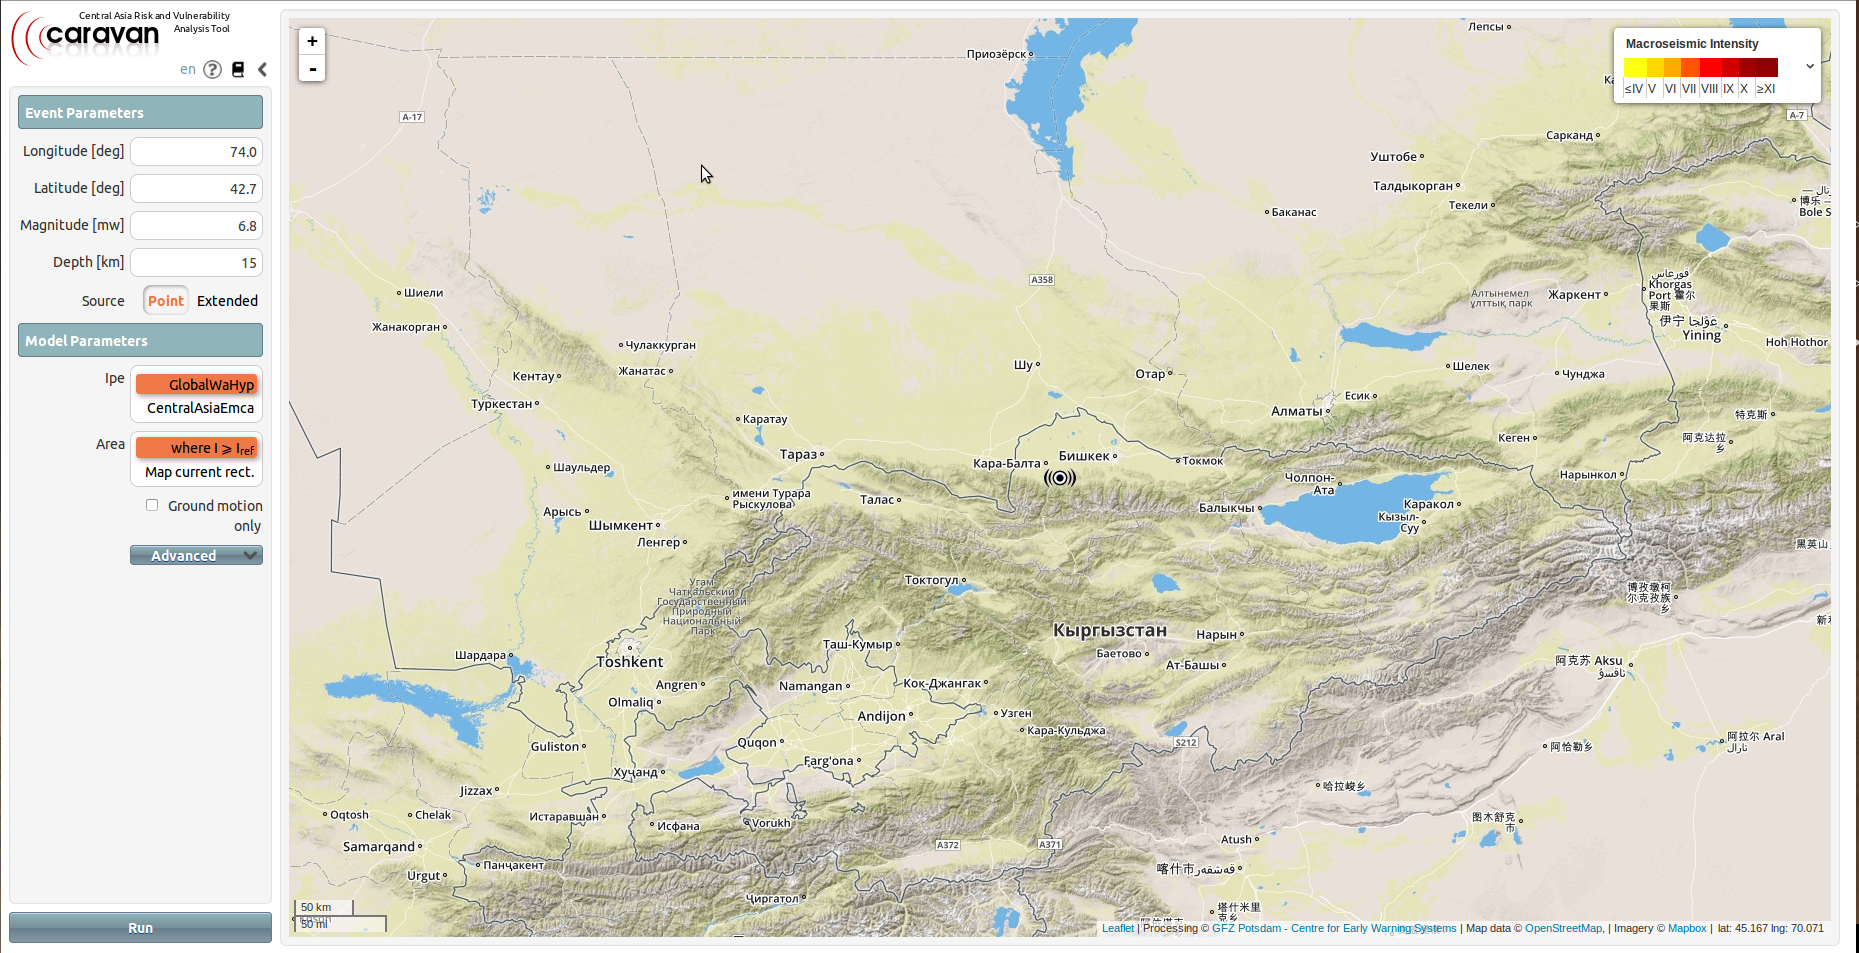
\includegraphics[width=\textwidth]{fig1}
	\captionof{figure}{Screenshot of the CARAVAN web application}
\end{center}

\subsection{Event parameters}
\emph{in construction}

\subsection{Model parameters}
\emph{in construction}

\subsection{FDSN event sources}
\emph{in construction}

\subsection{Interactive map}


\section{Scenario Impact computation}


\section{The CARAVAN Data Model}
\emph{in construction}





\end{document}
